% =====================================================================
% Evaluation section (INFOCOM). Requires: \usepackage{booktabs,graphicx}.
% Detection rate = fraction of ground-truth signals with box coverage >= 0.1.
% SNR is calibrated once on the 0 dB capture (in-box peak vs. pre-preamble noise
% in the same band) and propagated as snr = snr0 - attenuation.
% All numbers are from the six-detector sweep over the 0-60 dB attenuation set.
% =====================================================================
\section{Evaluation}
\label{sec:eval}

We evaluate six detectors that span three design philosophies: two deployed
detectors (\emph{coherent\_power}, a coherent power-integration detector, and
\emph{zero\_shot\_dino}, a frozen DINOv3 backbone applied zero-shot), two classical
non-learned baselines (\emph{3dB\_power}, a moving-average power threshold, and
\emph{blob\_detection}, an edge-and-blob image pipeline), and two fine-tuned learned
detectors (\emph{yolo}, a fine-tuned YOLO detector, and \emph{dino\_finetuned}, a
DINOv3 backbone with a fine-tuned segmentation head and lightly fine-tuned final
transformer blocks). Every detector emits a binary
time--frequency mask on an identical spectrogram grid and is scored by a single
evaluation pipeline against SigMF ground truth, so all comparisons are strictly
apples-to-apples.

We report results on a physically meaningful \emph{signal-to-noise ratio} (SNR) axis
rather than raw attenuation. SNR is calibrated once on the highest-power (0\,dB)
capture---per signal, the in-box peak power relative to the noise floor measured in
the same frequency band just before the burst's preamble---and propagated to every
attenuation step as $\mathrm{SNR}(A)=\mathrm{SNR}_0-A$, exploiting the fact that a
calibrated attenuator lowers the signal $1{:}1$ while the receiver noise floor is
unchanged. This lets us compare a wideband 5G burst and a narrowband FM tone on the
same physical axis, which raw attenuation does not.

\subsection{Quantitative Results}
\label{sec:eval:quant}

\paragraph{Detection rate vs.\ SNR.}
Figure~\ref{fig:rate_vs_snr} plots region detection rate against SNR for all signals.
The fine-tuned learned detectors dominate the low-SNR regime: at
$\mathrm{SNR}\in[-10,5)$\,dB, \emph{dino\_finetuned} and \emph{yolo} detect
$58.4\%$ and $62.6\%$ of signals respectively, whereas \emph{coherent\_power} manages
only $3.2\%$ and \emph{zero\_shot\_dino} $8.5\%$. As SNR increases the deployed
detectors recover strongly---\emph{coherent\_power} rises to $76.8\%$ at mid SNR and
$95.9\%$ at high SNR ($[20,40)$\,dB)---while \emph{dino\_finetuned} remains the most
capable throughout, reaching $93.8\%$ and $99.2\%$. The overall ordering
(Table~\ref{tab:detrate}) is \emph{dino\_finetuned} ($71.0\%$) $>$
\emph{coherent\_power} ($66.1\%$) $\approx$ \emph{yolo} ($65.5\%$) $\approx$
\emph{blob\_detection} ($65.6\%$) $>$ \emph{zero\_shot\_dino} ($54.8\%$), with
\emph{3dB\_power} nominally at $100\%$---a figure we show below to be an artifact of
its false-positive behavior rather than genuine selectivity.

\paragraph{Frame-level accuracy and the 3\,dB false-positive trap.}
Figure~\ref{fig:frame_metrics} and Table~\ref{tab:pixel} report frame-level pixel
metrics. \emph{3dB\_power} attains the highest recall ($0.754$) but the second-lowest
precision ($0.329$) and by far the largest false-positive area
($\mathrm{FP}_{\text{area}}=0.205$, i.e.\ it flags $\sim\!20\%$ of the non-signal
time--frequency plane). Its ``$100\%$ detection rate'' is therefore a direct
consequence of indiscriminate firing: any coverage-based detection criterion is
trivially satisfied by a detector that lights up most of the spectrum. This is the
central caution of our study---detection rate alone is misleading, and must be read
jointly with false-positive area. In stark contrast, \emph{dino\_finetuned} achieves
the best precision ($0.937$), IoU ($0.689$), and F1 ($0.756$) at a negligible
false-positive area of $0.003$ ($68\times$ lower than \emph{3dB\_power}), and
\emph{yolo} is a close second ($\mathrm{P}=0.758$, F1$=0.740$,
$\mathrm{FP}_{\text{area}}=0.015$). \emph{coherent\_power} is precise and clean
($\mathrm{P}=0.658$, $\mathrm{FP}_{\text{area}}=0.019$) but its lower recall ($0.561$)
reflects the missed low-SNR signals seen in Fig.~\ref{fig:rate_vs_snr}.

\paragraph{Breakdowns and outliers.}
Table~\ref{tab:detrate} decomposes detection rate by bandwidth, pulse duration, and
signal class, exposing several instructive outliers.
\begin{itemize}
  \item \textbf{YOLO collapses on narrowband tones.} \emph{yolo} detects only
    $4.5\%$ of \emph{Narrowband\_FM} signals and $44.9\%$ of ${<}2$\,MHz-bandwidth
    signals, despite leading on wideband classes (5G downlink $72.9\%$, OFDM
    $73.2\%$). An axis-aligned box regressor trained predominantly on wideband,
    structured emissions has weak priors for thin, low-time-bandwidth-product tones,
    which occupy few pixels and lack the internal texture the detector keys on. This
    class-conditional brittleness foreshadows the out-of-distribution failure in
    Sec.~\ref{sec:eval:qual}.
  \item \textbf{Classical blob detection is complementary, not competitive.}
    \emph{blob\_detection} is \emph{best} on exactly the signals YOLO misses---
    \emph{Narrowband\_FM} $96.5\%$, \emph{Broadband\_FM} $92.4\%$, ${<}2$\,MHz
    $94.8\%$---because sharp-edged, high-contrast tones are ideal for an edge/blob
    operator, but it degrades badly on wideband modulated traffic (5G $44.7\%$,
    $10$--$25$\,MHz $44.5\%$) whose diffuse energy lacks clean edges.
  \item \textbf{Coherent power needs dwell time.} \emph{coherent\_power} is weakest on
    the shortest bursts (${<}10$k samples: $41.1\%$, its lowest cell) because coherent
    integration requires sufficient on-time to accumulate SNR; the learned detectors,
    which reason over spatial appearance rather than integration gain, degrade far
    less ($59.0\%$ for \emph{dino\_finetuned}).
  \item \textbf{Fine-tuning is what makes DINO work.} \emph{zero\_shot\_dino} is
    uniformly mediocre (precision $0.231$, $\mathrm{FP}_{\text{area}}=0.114$): a
    frozen, natural-image backbone produces features that are not calibrated to RF
    spectrograms. Fine-tuning the same backbone lifts precision to $0.937$ and
    quadruples IoU, isolating the value of task adaptation from the value of the
    architecture.
\end{itemize}
Across all cells, \emph{dino\_finetuned} shows the flattest profile (no class below
$63\%$, no catastrophic bandwidth or duration failure), evidencing a detector whose
competence is broad rather than concentrated on the modalities best represented in
training.

% ---------- wide detection-rate table ----------
\begin{table*}[t]
\centering
\caption{Region detection rate (\% of ground-truth signals with box coverage
$\ge 0.1$), by SNR band and by signal category. Best legitimate detector per row in
\textbf{bold}. \emph{3dB\_power}'s uniformly $100\%$ column is an artifact of its
$\sim\!20\%$ false-positive area (Table~\ref{tab:pixel}), not selectivity, and is
excluded from the bolding ($\dagger$).}
\label{tab:detrate}
\begin{tabular}{@{}l r r r r r r@{}}
\toprule
 & Coherent & Zero-shot & 3dB & Blob & YOLO & DINO \\
 & power & DINO & power$^{\dagger}$ & detect. & & (FT) \\
\midrule
\multicolumn{7}{@{}l}{\textit{Overall detection rate vs.\ SNR}}\\
\quad Low SNR $[-10,5)$\,dB   & 3.2  & 8.5  & 100 & 6.7  & \textbf{62.6} & 58.4 \\
\quad Mid SNR $[5,20)$\,dB    & 76.8 & 55.9 & 100 & 63.7 & 83.9 & \textbf{93.8} \\
\quad High SNR $[20,40)$\,dB  & 95.9 & 91.3 & 100 & 77.2 & 85.2 & \textbf{99.2} \\
\quad All SNR                 & 66.1 & 54.8 & 100 & 65.6 & 65.5 & \textbf{71.0} \\
\midrule
\multicolumn{7}{@{}l}{\textit{By occupied bandwidth (all SNR)}}\\
\quad ${<}2$\,MHz    & 74.2 & 60.3 & 100 & \textbf{94.8} & 44.9 & 74.4 \\
\quad $2$--$10$\,MHz & 69.3 & 59.3 & 100 & 49.2 & \textbf{75.6} & 72.3 \\
\quad $10$--$25$\,MHz& 62.5 & 51.2 & 100 & 44.5 & \textbf{74.8} & 67.8 \\
\quad $25$--$60$\,MHz& 58.1 & 46.3 & 100 & 47.1 & \textbf{67.2} & 64.7 \\
\quad ${\ge}60$\,MHz & 54.5 & 46.6 & 100 & 66.2 & \textbf{75.9} & 68.9 \\
\midrule
\multicolumn{7}{@{}l}{\textit{By pulse duration (all SNR)}}\\
\quad ${<}10$k         & 41.1 & 47.1 & 100 & \textbf{78.9} & 52.9 & 59.0 \\
\quad $10$k--$100$k    & 75.1 & 58.8 & 100 & \textbf{87.4} & 59.3 & 68.2 \\
\quad $100$k--$1$M     & 69.6 & 58.8 & 100 & \textbf{83.3} & 64.0 & 69.8 \\
\quad $1$M--$5$M       & 68.6 & 54.7 & 100 & 53.9 & 69.9 & \textbf{74.4} \\
\midrule
\multicolumn{7}{@{}l}{\textit{By signal class (all SNR)}}\\
\quad Narrowband\_FM & 81.4 & 53.2 & 100 & \textbf{96.5} & 4.5  & 72.1 \\
\quad Broadband\_FM  & 62.4 & 62.9 & 100 & \textbf{92.4} & 51.3 & 74.2 \\
\quad Bluetooth      & 73.9 & 61.2 & 100 & \textbf{85.7} & 77.3 & 74.6 \\
\quad 802.11ax       & 57.8 & 46.7 & 100 & 55.0 & \textbf{68.2} & 63.1 \\
\quad 5G\_Downlink   & 63.0 & 48.4 & 100 & 44.7 & \textbf{72.9} & 68.4 \\
\quad OFDM           & 59.8 & 49.9 & 100 & 65.8 & \textbf{73.2} & 66.4 \\
\quad QPSK           & 67.7 & 57.0 & 100 & 67.6 & 62.9 & \textbf{72.9} \\
\quad BPSK           & 68.0 & 57.0 & 100 & 67.6 & 62.7 & \textbf{72.4} \\
\quad 16QAM          & 66.8 & 57.4 & 100 & 70.6 & 64.1 & \textbf{72.5} \\
\bottomrule
\end{tabular}
\end{table*}

% ---------- frame-level pixel-metric table ----------
\begin{table}[t]
\centering
\caption{Frame-level pixel metrics averaged over all frames. Best in \textbf{bold}.
$\mathrm{FP}_{\text{area}}$ is the fraction of non-signal area falsely flagged; lower
is better.}
\label{tab:pixel}
\begin{tabular}{@{}l c c c c c@{}}
\toprule
Detector & Prec. & Recall & F1 & IoU & $\mathrm{FP}_{\text{area}}\!\downarrow$ \\
\midrule
coherent\_power  & 0.658 & 0.561 & 0.543 & 0.389 & 0.019 \\
zero\_shot\_dino & 0.231 & 0.395 & 0.248 & 0.138 & 0.114 \\
3dB\_power       & 0.329 & \textbf{0.754} & 0.436 & 0.281 & 0.205 \\
blob\_detection  & 0.405 & 0.515 & 0.402 & 0.247 & 0.055 \\
yolo             & 0.758 & \textbf{0.766} & 0.740 & 0.611 & 0.015 \\
dino\_finetuned  & \textbf{0.937} & 0.732 & \textbf{0.756} & \textbf{0.689} & \textbf{0.003} \\
\bottomrule
\end{tabular}
\end{table}

\begin{figure}[t]
  \centering
  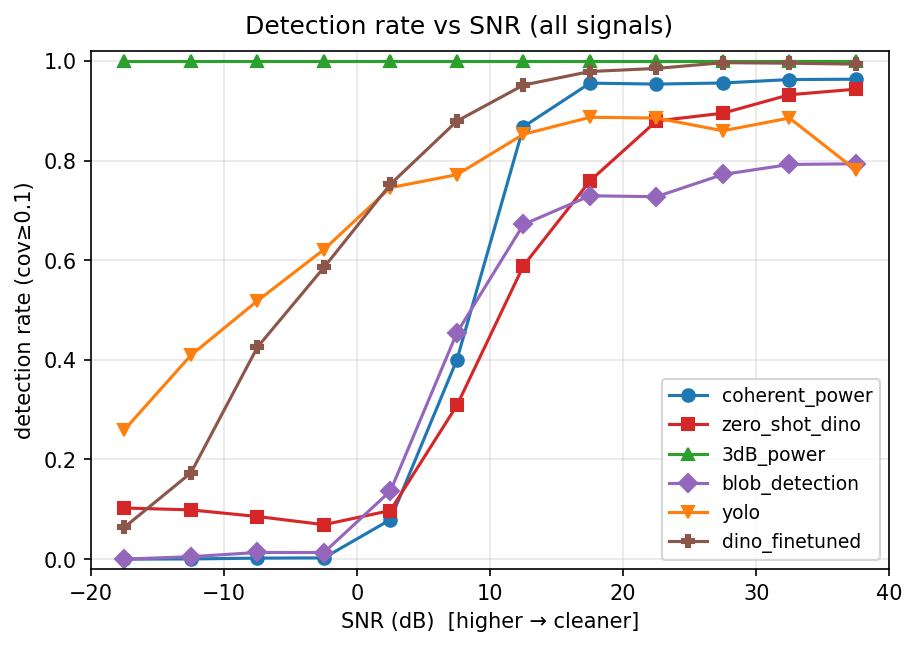
\includegraphics[width=\columnwidth]{figs/rate_vs_snr_overall.png}
  \caption{Detection rate vs.\ SNR, all signals. The fine-tuned detectors dominate
  the low-SNR regime; \emph{coherent\_power} recovers at high SNR;
  \emph{3dB\_power}'s flat $100\%$ reflects false-positive flooding
  (cf.\ Fig.~\ref{fig:frame_metrics}).}
  \label{fig:rate_vs_snr}
\end{figure}

\begin{figure*}[t]
  \centering
  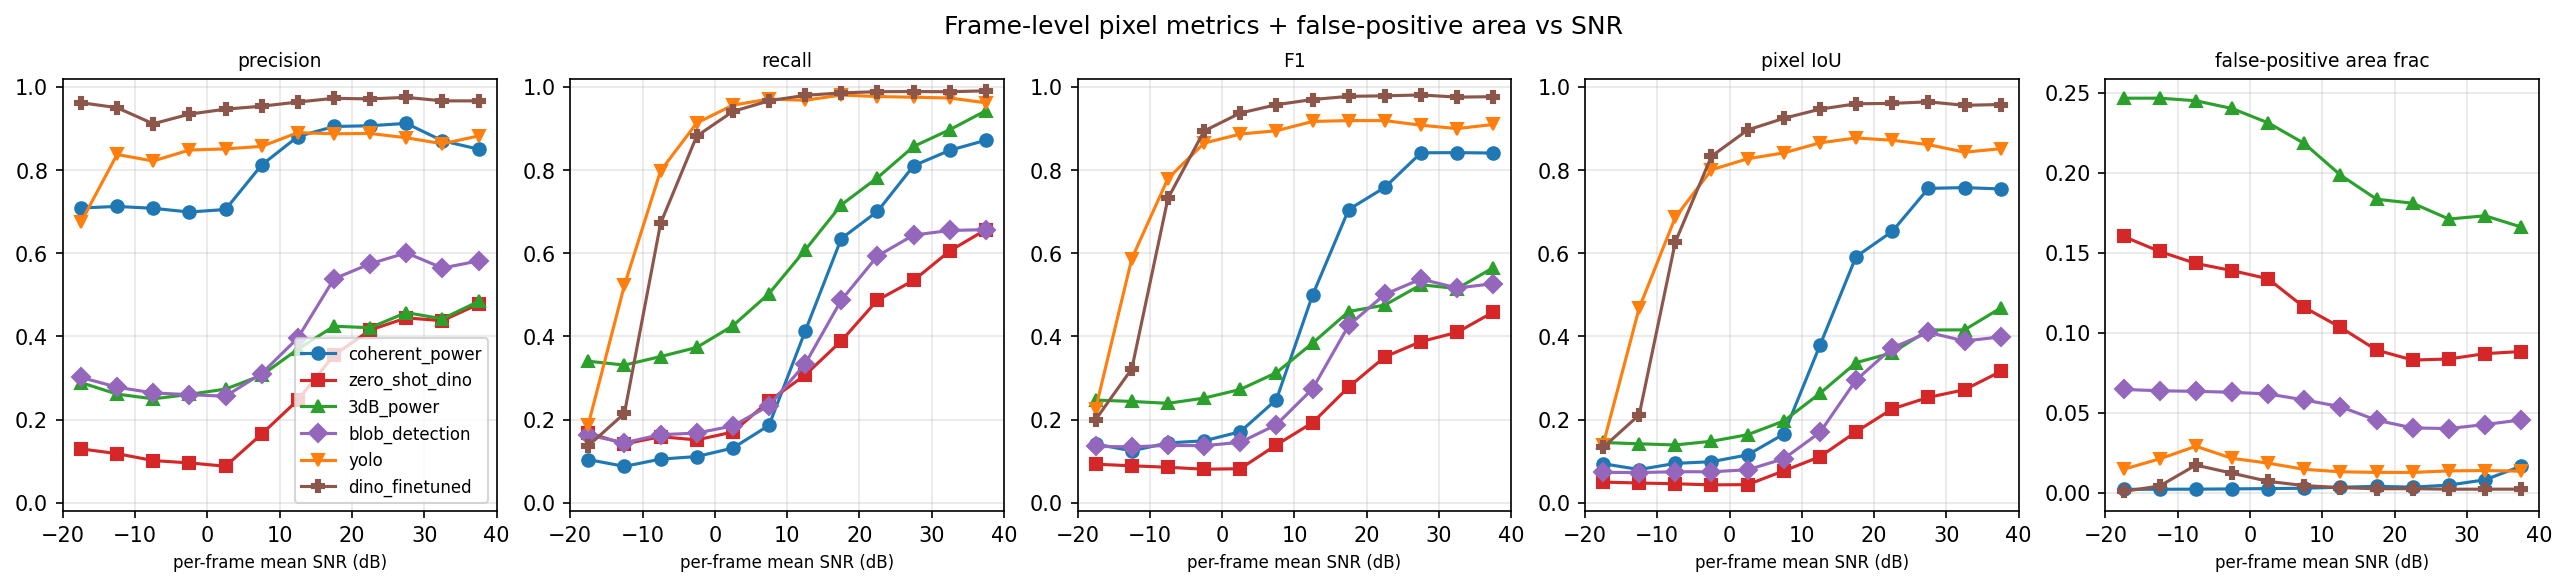
\includegraphics[width=\textwidth]{figs/frame_metrics_vs_snr.png}
  \caption{Frame-level precision, recall, F1, IoU, and false-positive area vs.\ SNR.
  \emph{dino\_finetuned} combines the highest precision/IoU with the lowest
  false-positive area; \emph{3dB\_power}'s high recall is paid for with a large
  false-positive area.}
  \label{fig:frame_metrics}
\end{figure*}

\subsection{Qualitative Results: In-Distribution and Over-the-Air}
\label{sec:eval:qual}

The controlled sweep above is in-distribution for the learned detectors. To probe
operational behavior we examine masks directly, both on the controlled captures and
on a live over-the-air (OTA) collection, \texttt{test\_1}: a wideband capture of the
2.4\,GHz ISM band containing a mixture of Wi-Fi, Bluetooth, and IoT emissions with
heavily varying bandwidths, duty cycles, and power levels---a regime the learned
detectors never saw in training.

\paragraph{Coherent power: the high-SNR, low-cost workhorse.}
On a controlled high-SNR frame (Fig.~\ref{fig:qual_controlled}) \emph{coherent\_power}
cleanly delineates every strong emission with tight, low-false-positive masks,
consistent with its $95.9\%$ high-SNR detection rate and $0.019$ false-positive area.
Its decisive practical advantage is cost: it is a fixed, non-learned integration with
negligible per-frame compute and no accelerator dependence, making it the detector of
choice when collection conditions guarantee adequate SNR and when latency and
processing budget are the binding constraints.

\paragraph{DINO fine-tuned: maximal sensitivity into low SNR.}
On \texttt{test\_1}, \emph{dino\_finetuned} is the strongest detector qualitatively:
it recovers every emission that \emph{coherent\_power} finds \emph{and} additionally
segments substantially weaker signals buried near the noise floor that coherent
integration misses. This mirrors the quantitative low-SNR gap
(Fig.~\ref{fig:rate_vs_snr}) and indicates that when the objective is maximal
detection capability into low-SNR regimes---and compute budget permits a learned
model---\emph{dino\_finetuned} is the premier choice, extending the usable detection
envelope well below what the deployed detectors reach.

\paragraph{YOLO under distribution shift.}
The most instructive OTA result is a \emph{failure}. Although \emph{yolo} is highly
competitive in-distribution (Table~\ref{tab:detrate}), on \texttt{test\_1}---which is
fully out-of-distribution (OOD)---it degrades sharply: it hallucinates coverage,
blocking out large contiguous swaths of spectrum where it grossly over-estimates
signal extent, while simultaneously missing obvious, clearly-present emissions. This
is the characteristic breakdown of a supervised, appearance-matching box detector
pushed off its training manifold.

\paragraph{Why DINO generalizes and YOLO does not.}
The divergence follows directly from the two models' architectures and learning
objectives. \emph{yolo} is a supervised object detector: it learns, discriminatively,
a mapping from local appearance to a small set of axis-aligned bounding boxes,
optimized end-to-end for the training distribution of shapes, bandwidths, and
duty-cycles. Its inductive biases---objectness priors, anchor/box regression, and
non-maximum suppression---encode strong assumptions about what a ``signal'' looks
like; when the ISM-band mixture violates those assumptions, the detector both
over-commits (fusing adjacent or extended emissions into one oversized box) and
under-detects (rejecting emissions that do not match learned box statistics). Its
representation is optimized to \emph{recognize the training set}, not to
\emph{describe the spectrum}.

\emph{dino\_finetuned}, by contrast, is a self-supervised representation with a light
task head. The DINOv3 backbone is pre-trained without labels to produce dense,
semantically structured, locally-consistent features that are known to transfer
robustly across domains; fine-tuning trains a lightweight segmentation head and gently
adapts only the last few transformer blocks at a reduced learning rate, leaving the
bulk of the self-supervised representation intact rather than reshaping it around a
narrow label set. Notably, a head-only variant with a fully frozen backbone performs
nearly as well, confirming that the transferable pretrained features---not the
fine-tuning---do most of the generalization work. Two properties follow. First, \emph{dense per-pixel segmentation} imposes no global shape
prior---each time--frequency cell is classified from its own rich context, so an
unfamiliar emission is described locally rather than forced into a learned box
template, avoiding both the block-out and the miss failure modes. Second, the
\emph{self-supervised feature manifold} is far broader than any labeled detection
set, so OOD spectra still land on meaningful features and the head degrades gracefully
rather than catastrophically. In short, YOLO's discriminative, box-centric objective
overfits to the appearance of the training distribution, whereas DINO's
self-supervised, dense-prediction design yields a representation that continues to
generalize when the input distribution shifts---exactly the property required for
robust wideband detection in the wild.

\begin{figure*}[t]
  \centering
  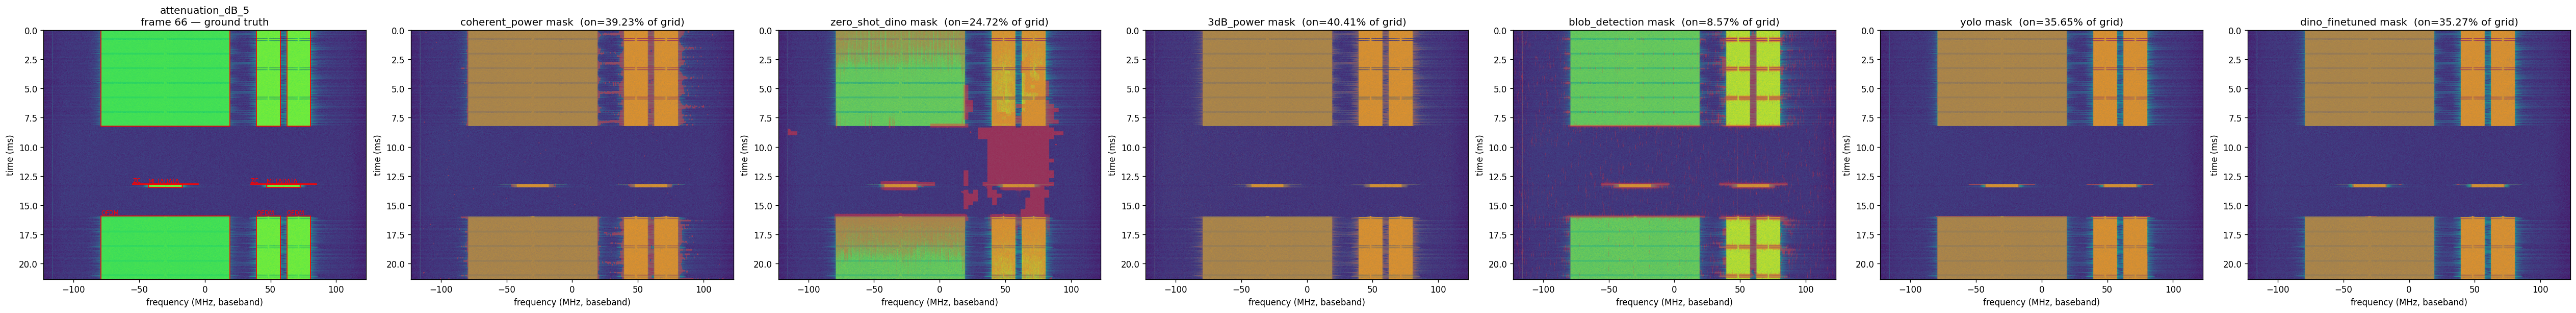
\includegraphics[width=\textwidth]{figs/qual_controlled.png}
  \caption{Controlled high-SNR frame (in-distribution), all six detectors. Panel~0
  is the spectrogram with ground-truth boxes; each remaining panel overlays one
  detector's mask. In-distribution, \emph{coherent\_power}, \emph{yolo}, and
  \emph{dino\_finetuned} all delineate the wideband emissions accurately;
  \emph{zero\_shot\_dino} is noisy and \emph{blob\_detection}, being edge-based,
  captures only signal boundaries---note that \emph{yolo} performs well \emph{here},
  in contrast to its out-of-distribution failure in Fig.~\ref{fig:qual_ota}.}
  \label{fig:qual_controlled}
\end{figure*}

\begin{figure*}[t]
  \centering
  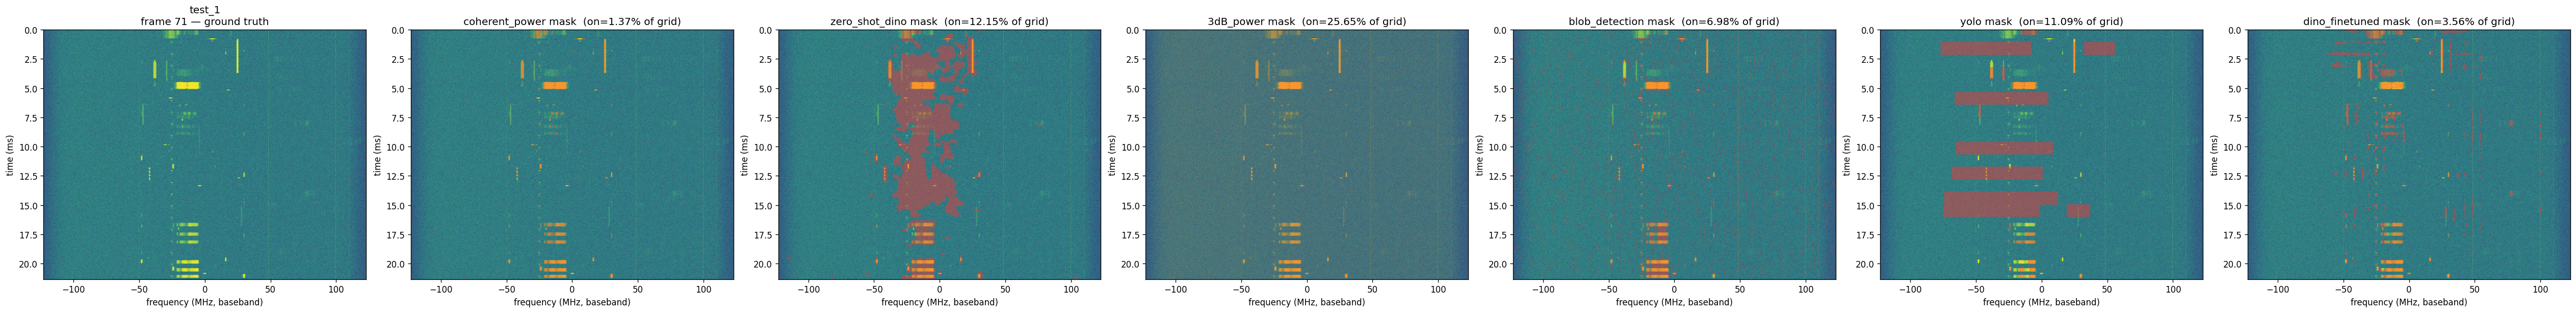
\includegraphics[width=\textwidth]{figs/ota_test1_panels.png}
  \caption{Out-of-distribution OTA capture \texttt{test\_1} (2.4\,GHz ISM: Wi-Fi /
  Bluetooth / IoT), all six detectors on one frame. \emph{coherent\_power} tightly
  marks the strong emissions; \emph{dino\_finetuned} captures those \emph{plus} the
  weaker narrowband cluster near the noise floor. \emph{yolo}, now off its training
  manifold, paints large false rectangular boxes across wide spectral spans while
  missing the fine narrowband signals; \emph{zero\_shot\_dino} and \emph{3dB\_power}
  flood the plane with false positives.}
  \label{fig:qual_ota}
\end{figure*}

\subsection{Discussion and Deployment Guidance}
\label{sec:eval:takeaways}

Three practical conclusions follow. \textbf{(i) Detection rate must never be reported
alone.} The \emph{3dB\_power} baseline achieves a perfect nominal detection rate while
falsely flagging one-fifth of the spectrum (Table~\ref{tab:pixel}); only the joint
view with false-positive area exposes it as unusable. We therefore advocate reporting
detection rate and false-positive area together, on a calibrated SNR axis.
\textbf{(ii) The right detector depends on the operating regime.} When SNR is
comfortably high and compute or latency is the binding constraint,
\emph{coherent\_power} is the pragmatic choice---$95.9\%$ high-SNR detection at
near-zero false-positive area and negligible cost. When the mission demands sensitivity
into low SNR and a learned model is affordable, \emph{dino\_finetuned} is the premier
detector, dominating precision, IoU, and low-SNR detection while extending the usable
envelope below where the deployed detectors operate. \textbf{(iii) Robustness to
distribution shift is an architectural property, not a training detail.} In-distribution,
\emph{yolo} is competitive; out-of-distribution it fails characteristically, because a
discriminative, box-centric objective encodes the training distribution's appearance
priors. \emph{dino\_finetuned}'s self-supervised, dense-prediction design generalizes to
the OTA ISM band with graceful degradation---precisely the behavior required for
open-world wideband sensing. Taken together, the fine-tuned DINO segmenter offers the
best overall capability and the most robust generalization, while coherent power remains
the efficient high-SNR workhorse; the classical and zero-shot baselines are useful
reference points but are not deployment-grade for wideband, low-SNR, or out-of-distribution
operation.
